t\climbingarea{Region 1}{%
This is the description for region 1.
\pgfplotscreateplotcyclelist{climbing}{
	{blue,fill=blue!30!white,mark=none},
    {red,fill=red!30!white,mark=none},
    {green,fill=green!60!white,mark=none}
}
\pgfplotsset{width=8cm,compat=1.17}
\def\chartone{%
  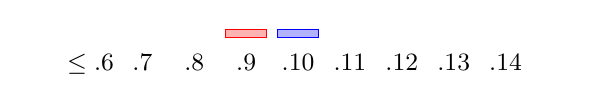
\begin{tikzpicture}
    \begin{axis}[
	    y=1mm,
	    axis lines=left,
		axis line style={draw=white},
        ybar stacked,
	    bar width=15pt,
        enlargelimits=0.15,
        symbolic x coords={$\leq.6$, .7, .8, .9, .10, .11, .12, .13, .14},
        xtick=data,
		xtick style={draw=none},
		ytick=\empty,
        x tick label style={font=\small},
    ]
	    \addplot+[ybar] plot coordinates {($\leq.6$,0) (.7,0) (.8,0) (.9,0) (.10,1) (.11,0) (.12,0) (.13,0) (.14,0)};
        \addplot+[ybar] plot coordinates {(.9,1)};
    \end{axis}
  \end{tikzpicture} 
}
\def\charttwo{%
  \begin{tikzpicture}
    \begin{axis}[
	    y=1mm,
	    axis x line=bottom,      % Show x-axis line at the bottom
        axis y line=none,        % Hide y-axis lines (left and right)
        axis line style={-},     % No arrowheads, just plain lines
        ybar stacked,
	    bar width=15pt,
        enlargelimits=0.15,
        symbolic x coords={${\leq}.6$, .7, .8, .9, .10, .11, .12, .13, .14},
        xtick=data,
        xtick style={draw=none},
        ytick=\empty,
        x tick label style={font=\scriptsize},
        ymin=0,
        enlarge y limits={abs=0}, % <-- removes the gap between bars and x-axis
		cycle list name=climbing,
    ]
	    \addplot coordinates {(${\leq}.6$,1) (.7,0) (.8,0) (.9,0) (.10,2) (.11,0) (.12,0) (.13,0) (.14,0)};
        \addplot coordinates {(${\leq}.6$,1) (.7,0) (.8,0) (.9,0) (.10,1)};
    \end{axis}
  \end{tikzpicture}
}
\climbingarea{First Wall}{%
    This is the description for the first wall.\\
    \begin{tabular}{c c c c} 
          \toprule
          Wall & Routes & Grades & Classics \\ 
          \midrule
          First Wall & 2 & \chartone&   \\ 
          \midrule
          Boulderfield Wall & 8 & \charttwo& Sporty McSportface \\ [1ex]
          \bottomrule
        \end{tabular}
    \climbheader{}{What is the access information}{How do you get there}{}
    }{%
        \tradroute[X]{The Trad Route Name}{5.9}{Use anchors on the next route.}{70}{Santa Claus}
        \sportroute{Sport Route Name}{5.10c}{Jug to the top.}{70}{5}{Jane Doe}
    }
    \climbingarea{Boulderfield Name}{%
        \climbheader{}{Access Info}{}{}
        \climbingarea{Big Rock}{%
            \climbheader{\lipsum[1][1]}{\lipsum[1][2-4]}{\lipsum[1][5-7]}{\lipsum[1][8]}% chktex 8
        }{%
            \boulderproblem{A Problem}{V3}{Problem Description}{10}{Alan Smithee}
            \tradroute{Another Fun Route}{5.10a}{Make sure the route numbers are not indented}{5}{Jolly Roger}
            \sportroute{Sporty McSportface}{5.10a}{\lipsum[1][9-10]}{5}{15}{Dr.\ Who}% chktex 8
            \boulderproblem{B Problem}{V0-}{\lipsum[1][11-12]}{15}{James Bond}% chktex 8
            \mixedtradroute{A Bolt or Two}{5.4}{\lipsum[1][13]}{100}{2}{Twista Bolten}
            \toproperoute{No Bolts}{5.6}{\lipsum[2][1-2]}{25}{Cher}% chktex 8
            \iceroute{Ice 9}{WI 2}{\lipsum[2][3-4]}{25}{Bobby Drake}% chktex 8
            \sportroute{Unknown Height}{5.10a}{Unit of measure of height should not be printed.}{}{15}{Mr.\ Bean}
        }
    }{}
}{}
